\documentclass[border=4pt]{standalone}
\usepackage{pgfplots}
\pgfplotsset{compat=1.18}

\begin{document}
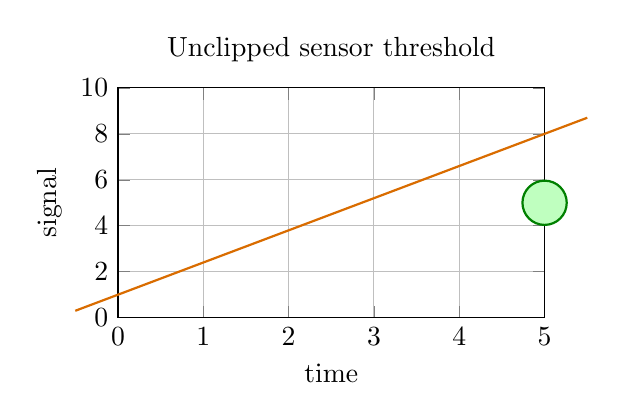
\begin{tikzpicture}
  \begin{axis}[
    width=7cm,
    height=4.5cm,
    xmin=0, xmax=5,
    ymin=0, ymax=10,
    enlargelimits=false,
    clip=false,
    clip mode=global,
    grid=major,
    title={Unclipped sensor threshold},
    xlabel={time}, ylabel={signal}
  ]
    \addplot[domain=-0.5:5.5,samples=25,orange!85!black,thick] {1.4*x+1};
    \filldraw[green!50!black,fill=green!25,thick] (axis cs:5,5) circle (8pt);
  \end{axis}
\end{tikzpicture}
\end{document}
